\section{Curve, Scalar Field and Vector Feild}

We must wander what is a geometry in our space. Is it a curve surface or a field? There are
two basic views on it. If we think of it as a curve surface, that is to say it's essence is beyond
our given space. \textit{(Later we'll call it as a submanifold embedded into our given space.)}
As a curve surface is two-dimensional, a point on the surface can be identified within two coordinates
$(u, v) \in C \subset \mathbb{R}^2$, where $C$ denotes a collection of points on the curve surface
and is a subset of $\mathbb{R}^2$. \textit{(We shall clarify what "ponits" actually mean later.)}
Now we only adopt an intrinsic perspective on the surface without observing it's curvature until we
use a \textbf{map} $\phi: C \to \mathbb{R}^3, (u,v) \mapsto (x,y,z)=\phi(u,v)$.

\begin{figure}[!ht]
    \centering
    \tikzset{every picture/.style={line width=0.75pt}} %set default line width to 0.75pt        

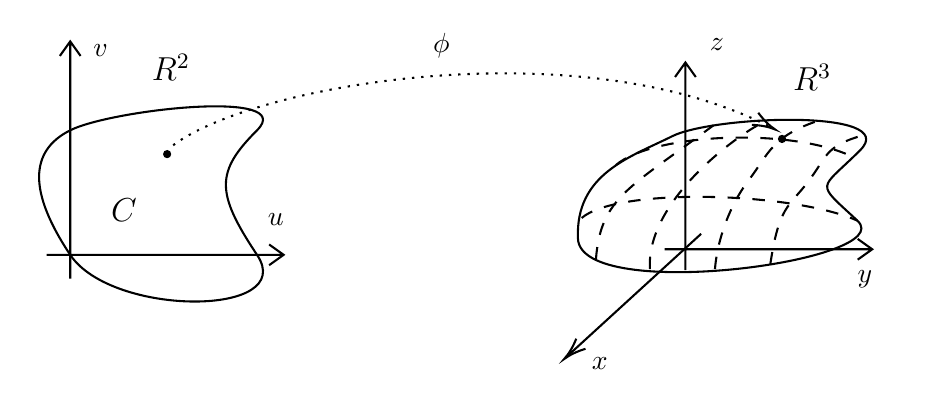
\begin{tikzpicture}[x=0.75pt,y=0.75pt,yscale=-1,xscale=1]
%uncomment if require: \path (0,310); %set diagram left start at 0, and has height of 310

%Shape: Polygon Curved [id:ds48992926630033473] 
\draw   (122,120) .. controls (142,110) and (232,100) .. (212,120) .. controls (192,140) and (192,150) .. (212,180) .. controls (232,210) and (142,210) .. (122,180) .. controls (102,150) and (102,130) .. (122,120) -- cycle ;
%Shape: Axis 2D [id:dp2965629103325713] 
\draw  (110.58,180) -- (224.82,180)(122,77.18) -- (122,191.42) (217.82,175) -- (224.82,180) -- (217.82,185) (117,84.18) -- (122,77.18) -- (127,84.18)  ;
%Shape: Axis 2D [id:dp5420346490627617] 
\draw  (408.4,177.33) -- (508.4,177.33)(418.4,87.33) -- (418.4,187.33) (501.4,172.33) -- (508.4,177.33) -- (501.4,182.33) (413.4,94.33) -- (418.4,87.33) -- (423.4,94.33)  ;
%Straight Lines [id:da7514964803526925] 
\draw    (425.96,169.89) -- (361.43,228.87) ;
\draw [shift={(359.96,230.22)}, rotate = 317.57] [color={rgb, 255:red, 0; green, 0; blue, 0 }  ][line width=0.75]    (10.93,-3.29) .. controls (6.95,-1.4) and (3.31,-0.3) .. (0,0) .. controls (3.31,0.3) and (6.95,1.4) .. (10.93,3.29)   ;
%Shape: Polygon Curved [id:ds6951808849645182] 
\draw   (411.96,122.89) .. controls (431.96,112.89) and (522.62,109.56) .. (502.62,129.56) .. controls (482.62,149.56) and (480.62,144.22) .. (501.29,163.56) .. controls (521.96,182.89) and (367.96,203.56) .. (366.62,172.22) .. controls (365.29,140.89) and (391.96,132.89) .. (411.96,122.89) -- cycle ;
%Curve Lines [id:da980778814237804] 
\draw  [dash pattern={on 4.5pt off 4.5pt}]  (375.29,182.22) .. controls (377.51,152.11) and (391.96,147.56) .. (431.96,117.56) ;
%Curve Lines [id:da5479602891033832] 
\draw  [dash pattern={on 4.5pt off 4.5pt}]  (401.29,186.89) .. controls (399.29,152.89) and (445.96,120.89) .. (454.62,116.89) ;
%Curve Lines [id:da6898603476087093] 
\draw  [dash pattern={on 4.5pt off 4.5pt}]  (432.62,186.89) .. controls (433.76,172.91) and (439.63,156.07) .. (449.07,143.78) .. controls (458.5,131.48) and (459.84,122.5) .. (483.96,114.89) ;
%Curve Lines [id:da9441978960398951] 
\draw  [dash pattern={on 4.5pt off 4.5pt}]  (459.29,184.56) .. controls (463.51,156.5) and (467.96,157.21) .. (477.4,144.92) .. controls (486.84,132.62) and (485.23,127.75) .. (503.9,122.42) ;
%Curve Lines [id:da5866336500737575] 
\draw  [dash pattern={on 4.5pt off 4.5pt}]  (368.4,162.25) .. controls (385.9,147.25) and (470.4,149.75) .. (501.29,163.56) ;
%Curve Lines [id:da6220068442378734] 
\draw  [dash pattern={on 4.5pt off 4.5pt}]  (384.9,136.75) .. controls (402.4,121.75) and (467.01,118.44) .. (497.9,132.25) ;
%Shape: Circle [id:dp15376632798085632] 
\draw  [fill={rgb, 255:red, 0; green, 0; blue, 0 }  ,fill opacity=1 ] (167.25,131.47) .. controls (167.25,130.68) and (167.9,130.03) .. (168.69,130.03) .. controls (169.49,130.03) and (170.13,130.68) .. (170.13,131.47) .. controls (170.13,132.27) and (169.49,132.92) .. (168.69,132.92) .. controls (167.9,132.92) and (167.25,132.27) .. (167.25,131.47) -- cycle ;
%Shape: Circle [id:dp39156470429151646] 
\draw  [fill={rgb, 255:red, 0; green, 0; blue, 0 }  ,fill opacity=1 ] (463.48,124.16) .. controls (463.48,123.36) and (464.13,122.71) .. (464.94,122.71) .. controls (465.74,122.71) and (466.39,123.36) .. (466.39,124.16) .. controls (466.39,124.97) and (465.74,125.62) .. (464.94,125.62) .. controls (464.13,125.62) and (463.48,124.97) .. (463.48,124.16) -- cycle ;
%Curve Lines [id:da06944123263869928] 
\draw  [dash pattern={on 0.84pt off 2.51pt}]  (171.6,127.2) .. controls (211.4,97.35) and (368.42,71.06) .. (460.22,118.87) ;
\draw [shift={(461.6,119.6)}, rotate = 208.05] [color={rgb, 255:red, 0; green, 0; blue, 0 }  ][line width=0.75]    (10.93,-3.29) .. controls (6.95,-1.4) and (3.31,-0.3) .. (0,0) .. controls (3.31,0.3) and (6.95,1.4) .. (10.93,3.29)   ;

% Text Node
\draw (215.67,158.4) node [anchor=north west][inner sep=0.75pt]    {$u$};
% Text Node
\draw (131.67,77.4) node [anchor=north west][inner sep=0.75pt]    {$v$};
% Text Node
\draw (499.87,186) node [anchor=north west][inner sep=0.75pt]    {$y$};
% Text Node
\draw (371.87,228) node [anchor=north west][inner sep=0.75pt]    {$x$};
% Text Node
\draw (428.67,74.4) node [anchor=north west][inner sep=0.75pt]    {$z$};
% Text Node
\draw (140.17,151.4) node [anchor=north west][inner sep=0.75pt]  [font=\large]  {$C$};
% Text Node
\draw (468.83,86.73) node [anchor=north west][inner sep=0.75pt]  [font=\large]  {$\mathbb{R}^{3}$};
% Text Node
\draw (159.83,81.9) node [anchor=north west][inner sep=0.75pt]  [font=\large]  {$\mathbb{R}^{2}$};
% Text Node
\draw (295.33,71.73) node [anchor=north west][inner sep=0.75pt]    {$\phi $};


\end{tikzpicture}
\caption{A map from $C$ to $\mathbb{R}^3$}
\end{figure}


\begin{figure}[!ht]
	\centering
    	

\tikzset{every picture/.style={line width=0.75pt}} %set default line width to 0.75pt        

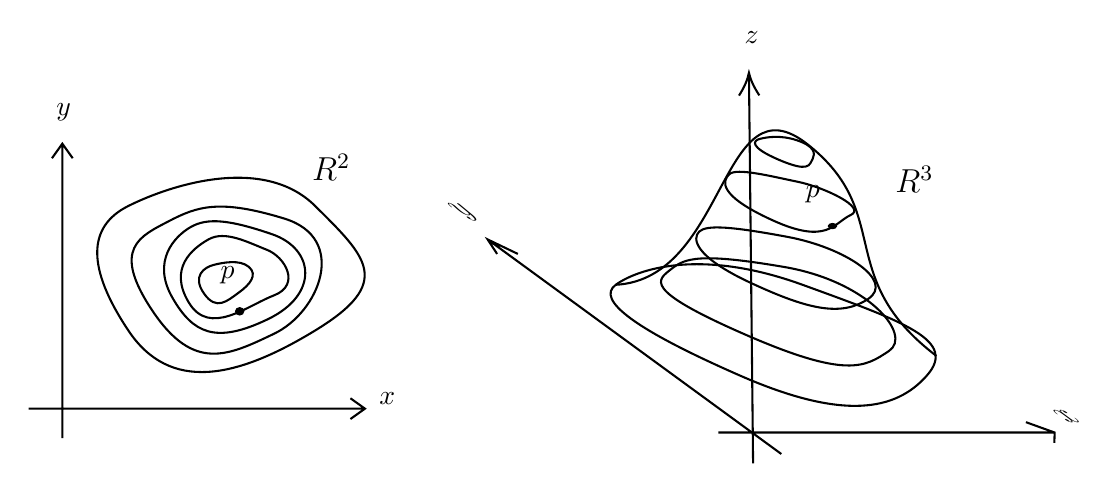
\begin{tikzpicture}[x=0.75pt,y=0.75pt,yscale=-1,xscale=1]
%uncomment if require: \path (0,300); %set diagram left start at 0, and has height of 300

%Shape: Axis 2D [id:dp15016489819991263] 
\draw  (84,209.65) -- (246,209.65)(100.2,82) -- (100.2,223.83) (239,204.65) -- (246,209.65) -- (239,214.65) (95.2,89) -- (100.2,82) -- (105.2,89)  ;
%Shape: Polygon Curved [id:ds27803715341113744] 
\draw   (132,112) .. controls (152,102) and (197,87.17) .. (222,112) .. controls (247,136.83) and (260,148.83) .. (222,172) .. controls (184,195.17) and (152,202) .. (132,172) .. controls (112,142) and (112,122) .. (132,112) -- cycle ;
%Straight Lines [id:da689974513691749] 
\draw    (433,236) -- (431.02,49.83) ;
\draw [shift={(431,47.83)}, rotate = 89.39] [color={rgb, 255:red, 0; green, 0; blue, 0 }  ][line width=0.75]    (10.93,-4.9) .. controls (6.95,-2.3) and (3.31,-0.67) .. (0,0) .. controls (3.31,0.67) and (6.95,2.3) .. (10.93,4.9)   ;
%Shape: Polygon Curved [id:ds31339915647514105] 
\draw   (151.5,119.33) .. controls (165.33,112.08) and (176.17,108.58) .. (207.17,118.08) .. controls (238.17,127.58) and (224.17,163.08) .. (202.17,173.58) .. controls (180.17,184.08) and (163.5,192.33) .. (143.5,162.33) .. controls (123.5,132.33) and (137.67,126.58) .. (151.5,119.33) -- cycle ;
%Shape: Polygon Curved [id:ds05477932375674843] 
\draw   (162.17,122.08) .. controls (170.17,117.58) and (180.67,118.58) .. (201.17,125.58) .. controls (221.67,132.58) and (224.17,154.58) .. (199.17,166.58) .. controls (174.17,178.58) and (163.17,173.58) .. (153.17,156.08) .. controls (143.17,138.58) and (154.17,126.58) .. (162.17,122.08) -- cycle ;
%Shape: Polygon Curved [id:ds8281269379162415] 
\draw   (170.67,128.08) .. controls (178.67,123.58) and (189.67,129.58) .. (198.67,133.08) .. controls (207.67,136.58) and (215.17,150.08) .. (202.17,155.08) .. controls (189.17,160.08) and (171.17,175.08) .. (161.17,158.58) .. controls (151.17,142.08) and (162.67,132.58) .. (170.67,128.08) -- cycle ;
%Shape: Polygon Curved [id:ds47537917404511076] 
\draw   (172.93,140.44) .. controls (177.19,139.36) and (185.59,137.56) .. (190.04,141.33) .. controls (194.48,145.11) and (190.7,149.78) .. (185.15,153.78) .. controls (179.59,157.78) and (174.44,162.69) .. (168.48,154.22) .. controls (162.52,145.75) and (168.67,141.53) .. (172.93,140.44) -- cycle ;
%Shape: Axis 2D [id:dp6952388440699333] 
\draw  (416.26,221.16) -- (578.29,221.16)(305.09,128.11) -- (446.61,231.5) (564.45,216.16) -- (578.29,221.16) -- (578.14,226.16) (309.67,135.11) -- (305.09,128.11) -- (319.67,135.11)  ;
%Shape: Polygon Curved [id:ds639624284886785] 
\draw   (366.83,149.98) .. controls (376.85,142.69) and (407.05,131.88) .. (456.83,149.98) .. controls (506.61,168.08) and (531.59,176.83) .. (516.71,193.72) .. controls (501.83,210.6) and (476.65,215.58) .. (426.71,193.72) .. controls (376.77,171.85) and (356.81,157.27) .. (366.83,149.98) -- cycle ;
%Shape: Polygon Curved [id:ds9876755207993106] 
\draw   (393.65,142.33) .. controls (400.25,137.04) and (407.59,134.49) .. (448.07,141.41) .. controls (488.55,148.34) and (509.98,174.22) .. (498.46,181.87) .. controls (486.94,189.52) and (478.51,195.54) .. (428.56,173.67) .. controls (378.62,151.8) and (387.05,147.61) .. (393.65,142.33) -- cycle ;
%Shape: Polygon Curved [id:ds15145527097429268] 
\draw   (407.06,124.33) .. controls (410.57,121.05) and (422.07,121.78) .. (449.55,126.88) .. controls (477.04,131.98) and (501.5,148.02) .. (488.47,156.77) .. controls (475.45,165.52) and (459.46,161.87) .. (431.99,149.11) .. controls (404.53,136.36) and (403.55,127.61) .. (407.06,124.33) -- cycle ;
%Shape: Polygon Curved [id:ds17242550394796763] 
\draw   (421.55,96.7) .. controls (425.06,93.42) and (442.05,97.8) .. (454.54,100.35) .. controls (467.03,102.9) and (488.01,112.74) .. (480,116.38) .. controls (471.99,120.03) and (468.96,130.96) .. (442.49,118.94) .. controls (416.02,106.91) and (418.04,99.98) .. (421.55,96.7) -- cycle ;
%Shape: Polygon Curved [id:ds5038591074357603] 
\draw   (436.14,79.71) .. controls (439.32,78.92) and (445.93,77.61) .. (454.14,80.36) .. controls (462.36,83.12) and (463.24,86.52) .. (461.67,89.43) .. controls (460.11,92.35) and (459.87,95.93) .. (445.45,89.76) .. controls (431.03,83.58) and (432.97,80.5) .. (436.14,79.71) -- cycle ;
%Curve Lines [id:da_19952820114301328] 
\draw    (366.83,149.98) .. controls (420.78,147.11) and (417.44,49.11) .. (459.44,82.44) .. controls (501.44,115.78) and (471.33,146.25) .. (521.33,184.25) ;
%Shape: Ellipse [id:dp7921984943858547] 
\draw  [fill={rgb, 255:red, 0; green, 0; blue, 0 }  ,fill opacity=1 ] (183.93,162.75) .. controls (183.93,161.91) and (184.7,161.23) .. (185.65,161.23) .. controls (186.6,161.23) and (187.36,161.91) .. (187.36,162.75) .. controls (187.36,163.59) and (186.6,164.27) .. (185.65,164.27) .. controls (184.7,164.27) and (183.93,163.59) .. (183.93,162.75) -- cycle ;
%Shape: Ellipse [id:dp5207115909478626] 
\draw  [fill={rgb, 255:red, 0; green, 0; blue, 0 }  ,fill opacity=1 ] (469.52,121.69) .. controls (469.55,121.13) and (470.34,120.69) .. (471.29,120.69) .. controls (472.23,120.69) and (472.98,121.13) .. (472.95,121.69) .. controls (472.92,122.24) and (472.13,122.69) .. (471.18,122.69) .. controls (470.23,122.69) and (469.49,122.24) .. (469.52,121.69) -- cycle ;

% Text Node
\draw (251.4,200.2) node [anchor=north west][inner sep=0.75pt]    {$x$};
% Text Node
\draw (95.8,61.4) node [anchor=north west][inner sep=0.75pt]    {$y$};
% Text Node
\draw (571.59,209) node [anchor=north west][inner sep=0.75pt]  [xslant=-1.61]  {$x$};
% Text Node
\draw (280.7,109.4) node [anchor=north west][inner sep=0.75pt]  [xslant=-1.46]  {$y$};
% Text Node
\draw (427.4,26.6) node [anchor=north west][inner sep=0.75pt]    {$z$};
% Text Node
\draw (219,85.4) node [anchor=north west][inner sep=0.75pt]  [font=\large]  {$\mathbb{R}^{2}$};
% Text Node
\draw (500,91.4) node [anchor=north west][inner sep=0.75pt]  [font=\large]  {$\mathbb{R}^{3}$};
% Text Node
\draw (174.93,139.84) node [anchor=north west][inner sep=0.75pt]    {$p$};
% Text Node
\draw (456.93,100.84) node [anchor=north west][inner sep=0.75pt]    {$p$};


\end{tikzpicture}
    \caption{A scalar field over $\mathbb{R}^2$}
\end{figure}


Another way to think of a geometry is \textbf{scalar field} $f: \mathbb{R}^2 \to \mathbb{R}, (x,y) \mapsto f(x,y)$
If we write this way: $z=f(x,y)$ where $z$ represents each scalar value onto each point $(x,y)$.
There is a relationship between $z$ and $(x,y)$ that can be written as $((x,y),z)$ or just $(x,y,z)$.
All such relationships constitude a set $\mathbb{R}^3=\mathbb{R}^2 \times \mathbb{R}$

However the relationship between $x,y,z$ can be wider given by $F(x,y,z)=0$. $F$ is a strange function that
can be considered as a constant scalar field. Before we use an simpler example to gain a deeper understanding of it,
let's clarify some terms in the context.

\begin{definition}[Relation]
	\cite{1}
	A relation is a subset of a finite Cartes	`ian power $A^n=A\times\cdots\times A$ of a given set $A$,
	i.e. a set of tuples $(a_1,\dots,a_n)$ of $n$ elements of $A$.

	A subset $R\subseteq A^n$ is called an $n$-place, or an $n$-ary, relation on $A$.
	The number \textbf{n} is called the \textbf{rank}, or \textbf{type}, of the relation $R$.
	The notation $R(a_1,\dots,a_n)$ signifies that $(a_1,\dots,a_n)\in R$.

	The set $A^n$ and the empty subset $\emptyset$ in $R^n$ are called, respectively, the \textbf{universal relation} and the \textbf{zero relation} of rank n on $A$.
	The diagonal of the set $A^n$, i.e. the set $\Delta={(a,a,\dots,a):a\in A}$ is called the \textbf{equality relation} on $A$.

\end{definition}

The set of all $n$-ary relations on $A$ is a \textbf{Boolean algebra} relative to the operations $\cup, \cap, '$.
An $(n+1)$-place relation $F$ on $A$ is called functional if for any elements $a_1,\dots,an, a,b$, from $A$
it follows from $F(a_1,\dots,a_n,a)$ and $F(a_1,\dots,a_n,b)$ that $a=b$.

\begin{definition}[Binary Relation]
	\cite{2}
	A binary relation is a predicate on a given set.
	A binary relation is a special case of a relation. Let $R \subseteq A \times A$.
	If $(a,b) \in R$, then one says that the element $a$ is in binary relation $R$ to the element $b$.
	An alternative notation for $(a,b) \in R$ is $aRb$.

	The empty subset $\emptyset$ in $A\times A$ and the set $A\times A$ itself are called, respectively,
	the nil relation and the universal relation in the set $A$.
	The diagonal of the set $A\times A$, i.e. the set $\Delta={(a,a):a\in A}$,
	is the \textbf{equality relation} or the \textbf{identity binary relation} in $A$.

\end{definition}

Let $R,R_1,R_2$ be binary relations in a set $A$. In addition to the set-theoretic operations of union $R_1\cup R_2$,
intersection $R_1\cap R_2$, and negation or complementation $R'=(A\times A)\backslash R$,
one has the inversion (also inverse, converse or transpose)
\[R^{-1}={(a,b):(b,a)\in R},\]
as well as the operation of multiplication (or composition):
\[R_1\circ R_2={(a,c)∈A\times A:(\exists b\in A)(aR_1b\ and\ bR_2c)}.\]

\begin{definition}[Mapping]
	\cite{3}
	In set theory mappings are special binary relations.A mapping $f$ from a set $A$ to a set $B$ is an (ordered) triple $f=(A,B,G_f)$
 	where $Gf\subset A\times B$ such that

	\begin{itemize}
		\item[(1)] if $(x,y)$ and $(x,y')\in G_f$ then $y=y'$, and
		\item[(2)] the projection $\pi_1(G_f)=\{x|(x,y)\in G_f\}=A.$
	\end{itemize}

	Condition (1) expresses that $f$ is single-valued. and condition (2) that it is defined on $A$.
	$A$ is the \textbf{domain}, $B$ is the \textbf{codomain}, and $G_f$ is the \textbf{graph} of the mapping. Therefore, in this setting, mappings are equal if and only if all three corresponding components (domain, codomain, and graph) are equal.
	
	The mapping is usually denoted as $f:A\to B$, and $a\mapsto f(a)$ where $f(a):=b\Leftrightarrow (a,b)\in G_f$ is the value of $f$ at $a$.

\end{definition}

If two mappings $f_1=(A_1,B_1,G_1)$ and $f_2=(A_2,B_2,G_2)$ satisfy $A_1\subset A_2$, $B_1\subset B_2$ and $G_1\subset G_2$
then $f_2$ is called an \textbf{extension} of $f_1$, and $f_1$ a \textbf{restriction} of $f_2$.
In this case, $f_1$ is often denoted as $f_2|A_1$ and, clearly, $f_1(a)=f_2(a)$ holds for all $a\in A_1$.



\subsection{Implicit Function and Implicit Equation}

\begin{center}
	\begin{tcolorbox}[colback=gray!10,%gray background
					  colframe=black,% black frame colour
					  width=12cm,% Use 8cm total width,
					  arc=1mm, auto outer arc,
					  boxrule=0.5pt,
					 ]
	Notice that functions to be talked below are always $C^{\infty}$ (smooth) without special illustration.
	\end{tcolorbox}
\end{center}

A function $f: \mathbb{R}\to\mathbb{R}, x\mapsto y=f(x)$ is a explicit function and scalar filed over $\mathbb{R}$.
$f$ has good properties that we can define a derivative over it:

\begin{definition}
	For a real-valued function $f\in C^{k}: \mathbb{R}\to\mathbb{R}$, the \textbf{derivative} on $x_0\in D(f)$ is defined by:
	\[
		\left.\frac{\mathrm{d}}{\mathrm{d}x}\right|_{x_0} f :=
		\lim_{\Delta x\to 0}\frac{f(x_0+\Delta x)-f(x_0)}{t},
	\]
	for $\Delta x\in\mathbb{R}$.
\end{definition}

\begin{definition}
	Construct a function $\frac{\mathrm{d}}{\mathrm{d}x}f: C^{k}\to\mathbb{R}$ satisfying:
	\[
		\left(\frac{\mathrm{d}}{\mathrm{d}x}f\right)(x_0) :=
		\left.\frac{\mathrm{d}}{\mathrm{d}x}\right|_{x_0} f.
	\]
	$\frac{\mathrm{d}}{\mathrm{d}x}f$ is called the \textbf{derivative function}.
	It is denoted as $\frac{\mathrm{d}}{\mathrm{d}x}f\equiv f'$ simultaneously when it is clear whom to take the derivative from (always $x$).
	It is also write as $\dot{f}$ when taking the derivative from $t$.
\end{definition}

There are abundant corollaries on the field of derivative and are needless to say more. Let's turn our attention to
scalar field over $\mathbb{R}^n$, and we'll define the \textbf{derivative operator} and \textbf{directional derivative}
as well as the \textbf{gradient}. And we'll further study their geometric significance in the next section.

\begin{definition} [Parital Derivative]
	Given a function $f: \mathbb{R}^n\to\mathbb{R}, \mathbf{x}=(x^1,\dots,x^n)\mapsto y=f(\mathbf{x})$. The limitation is defined as the \textbf{partial derivative} at $\mathbf{x_0}$:
	\[
		\left.\frac{\partial}{\partial x^i}\right|_{\mathrm{x_0}} f:=
		\lim_{\Delta x^i\to 0}\frac{f(\dots,x_0^i+\Delta x^i,\dots)-f(\mathbf{x_0})}{\Delta x^i}=
		\left.\frac{\mathrm{d}}{\mathrm{d}x^i}\right|_{x^i=x_0^i\atop\Delta x^i=0} f(x_0^1,\dots,x^i,\dots,x_0^n).
	\]
\end{definition}

\begin{definition}
	\[
		\left(\frac{\partial}{\partial x^i}f\right)(\mathbf{x_0}):=
		\left.\frac{\partial}{\partial x^i}\right|_{\mathrm{x_0}} f
	\]
\end{definition}

\begin{theorem}[Chain Rule]
	Given a function $f: \mathbb{R}^n\to\mathbb{R}^m, \mathbf{x}\mapsto\mathbf{y}=f(\mathbf{x})$ that eats n variables and spit out m variables where $\mathbf{x}=(x^1,\dots,x^n), \mathbf{y}=(y^1,\dots,y^m)$.
	It can be thought of a vector $\langle f_1,\dots,f_n\rangle$ in which $f_i: \mathbb{R}\to\mathbb{R}^m, \mathbf{x}\mapsto y^i=f(\mathbf{x})$.
	All partial derivatives can be written in a maritx, which we called a \textbf{partial derivative tensor}:
	\[
		\frac{\partial f_j}{\partial x^i} = 
		\begin{bmatrix}
			\frac{\partial f_1}{\partial x^1} & \cdots & \frac{\partial f_1}{\partial x^n} \\
			\vdots & \ddots & \vdots \\
			\frac{\partial f_m}{\partial x^1} & \cdots & \frac{\partial f_m}{\partial x^n}
		\end{bmatrix}.
	\]
	Now we use vectors to represent a function chain: $\mathbf{z}=g(\mathbf{y}), \mathbf{y}=f(\mathbf{x})$. Then $\mathbf{z}=g(f(\mathbf{x}))=(g\circ f)(\mathbf{x})$. As can vertify,
	The partial derivative tensor of $z$ over $x$ is (here $z=g\circ f$ also):
	\[
		\frac{\partial z^k}{\partial x^i} = \frac{\partial g_k}{\partial y^j}\frac{\partial f_j}{\partial x^i},
	\]
	which is called the \textbf{Chain Rule}.
\end{theorem}

The partial derivative tensor written above is also a \textbf{Jacobian Matrix} of a vector-valued function. But isn't it better to take tensor notation?
When so, the gradient of each components can be represent more concise and intuitive!
\[
	D\vec{f} = \nabla f_j = \frac{\partial f_j}{\partial x^i}.
\]

\begin{example}
	\begin{itemize}
		\item[(1)] Calculate the gradient of $f(x,y)=\sin(xy)+\frac{x^2}{1+\ln y}$ at $(\pi,1)$.
		\begin{solution}
			$\frac{\partial f}{\partial x} = y\cos(xy)+\frac{2x}{1+\ln y},
			\quad \frac{\partial f}{\partial y} = x\cos(xy)-\frac{x^2}{y(1+\ln y)^2}$.

			Then $\nabla f|_{(\pi,1)}=(\left.\frac{\partial f}{\partial x}\right|_{(\pi,1)}, \left.\frac{\partial f}{\partial y}\right|_{(\pi,1)})=
			(-1+2\pi, -\pi-\pi^2)$.
		\end{solution}
		\item[(2)] Given a composite function $z=f(x+y^2, ye^x)$, calculate $\frac{\partial z}{\partial x}$.
		\begin{solution}
			Denote that $z=f(u,v)=f(u^1(x,y),u^2(x,y))$. According to the Chain Rule:
		
			$\frac{\partial z}{\partial x}=\frac{\partial f}{\partial u^i}\frac{\partial u^i}{\partial x}=\frac{\partial f}{\partial u^1}+\frac{\partial f}{\partial u^2}ye^x$.
		\end{solution}
	\end{itemize}
\end{example}

\begin{definition}[Derivative Operator]
	For a scalar field $f: \mathbb{R}^n\to\mathbb{R}$, consider a vector in $\mathbb{R}^n$: $\mathbf{v}=\langle v^1,\dots,v^n\rangle$.
	Define a coordinate function $x: p\mapsto \mathbf{x}=x(p)\in\mathbb{R}^n$, which can be determined by $x^i: p\mapsto x^i=x^i(p)\in\mathbb{R}$, $\mathbf{x}=(x^1,\dots,x^n)$.
	Then the coordinate of a neighbor in $\mathbf{v}$ direction can be determined by a function $c(t)=\mathbf{x}+t\mathbf{v}=(x^1+tv^1,\dots,x^n+tv^n)$.

	The \textbf{derivative operator} $D_{v,x_0}: C^{k}\to\mathbb{R}$ over $p$ is a map satisfying:
	\[
		D_{v,p}f := \lim_{t\to 0}\frac{f(c(t))-f(\mathbf{x})}{t} =
		\left.\frac{\mathrm{d}}{\mathrm{d} t}\right|_{t=0} (f\circ c)
	\]
\end{definition}

By using the Chain Rule, we get $\left.\frac{\mathrm{d}}{\mathrm{d} t}\right|_{t=0} (f\circ c) = v^i \left.\frac{\partial}{\partial x^i}\right|_{p} f$.
Since this is established for $\forall x_0 \in D(f)$, we obtain:
$D_{v}f = v^i \cdot \left(\frac{\partial}{\partial x^i}f\right)$.

\begin{definition}[Directional Derivative]
	Construct a function $D_vf: D(f)\to\mathbb{R}$ that satisfies:
	\[
		D_{v}f := v^i\cdot \left(\frac{\partial}{\partial x^i}f\right), \quad
		\left.D_vf\right|_p := v^i\cdot \left.\frac{\partial}{\partial x^i}\right|_p f.
	\]
	This means the \textbf{directional derivative} in the direction of $\mathbf{v}$.
\end{definition}

At Figure \ref{dirder} we can see that $\left\{\left.\frac{\partial}{\partial x^i}\right|_p\right\}$ spans a vector space as is easy to prove.
And if we construct a map from a vector $\mathbf{v}$ to the partial derivatives at point $p$, we can prove that the map is a algebraic isomorphism!
That means we can consider a vector



\begin{figure}[!ht]
	\centering
    

\tikzset{every picture/.style={line width=0.75pt}} %set default line width to 0.75pt        

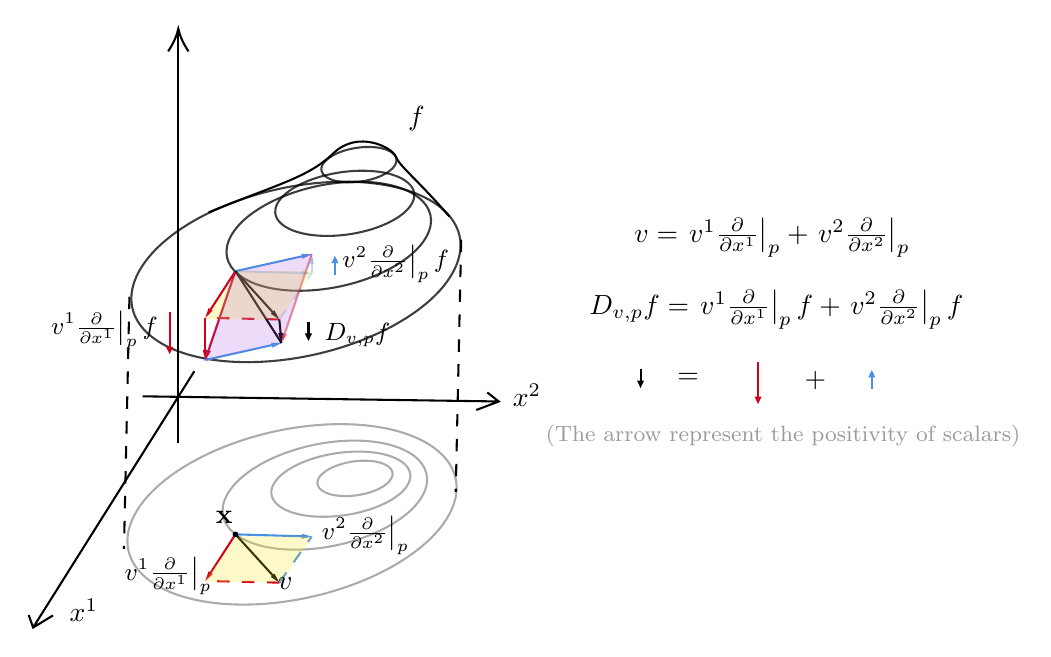
\begin{tikzpicture}[x=0.75pt,y=0.75pt,yscale=-1,xscale=1]
%uncomment if require: \path (0,324); %set diagram left start at 0, and has height of 324

%Shape: Axis 2D [id:dp392022965918875] 
\draw  (233.79,180.44) -- (156.1,303.95)(380.45,195.03) -- (208.86,192.55) (165.68,298.11) -- (156.1,303.95) -- (153.98,297.94) (374.92,190.68) -- (380.45,195.03) -- (369.6,199.15)  ;
%Straight Lines [id:da6093238245580039] 
\draw    (226.05,214.91) -- (226.05,17.44) ;
\draw [shift={(226.05,15.44)}, rotate = 90] [color={rgb, 255:red, 0; green, 0; blue, 0 }  ][line width=0.75]    (10.93,-4.9) .. controls (6.95,-2.3) and (3.31,-0.67) .. (0,0) .. controls (3.31,0.67) and (6.95,2.3) .. (10.93,4.9)   ;
%Shape: Ellipse [id:dp405330952821648] 
\draw  [color={rgb, 255:red, 0; green, 0; blue, 0 }  ,draw opacity=0.33 ][line width=0.75]  (205.09,249.42) .. controls (218.03,225.42) and (262.43,205.96) .. (304.26,205.96) .. controls (346.1,205.96) and (369.52,225.42) .. (356.59,249.42) .. controls (343.65,273.43) and (299.25,292.89) .. (257.41,292.89) .. controls (215.58,292.89) and (192.15,273.43) .. (205.09,249.42) -- cycle ;
%Shape: Ellipse [id:dp329912503849465] 
\draw  [color={rgb, 255:red, 0; green, 0; blue, 0 }  ,draw opacity=0.33 ][line width=0.75]  (249.46,240.15) .. controls (257.28,225.64) and (284.74,213.88) .. (310.81,213.88) .. controls (336.87,213.88) and (351.65,225.64) .. (343.84,240.15) .. controls (336.02,254.66) and (308.55,266.43) .. (282.49,266.43) .. controls (256.43,266.43) and (241.64,254.66) .. (249.46,240.15) -- cycle ;
%Shape: Ellipse [id:dp1514768215459963] 
\draw  [color={rgb, 255:red, 0; green, 0; blue, 0 }  ,draw opacity=0.33 ][line width=0.75]  (271.95,234.87) .. controls (276.62,226.2) and (294.92,219.17) .. (312.82,219.17) .. controls (330.72,219.17) and (341.44,226.2) .. (336.77,234.87) .. controls (332.09,243.54) and (313.79,250.58) .. (295.89,250.58) .. controls (277.99,250.58) and (267.27,243.54) .. (271.95,234.87) -- cycle ;
%Shape: Ellipse [id:dp668836996840452] 
\draw  [color={rgb, 255:red, 0; green, 0; blue, 0 }  ,draw opacity=0.33 ][line width=0.75]  (293.63,232.09) .. controls (296.17,227.38) and (306.09,223.57) .. (315.78,223.57) .. controls (325.48,223.57) and (331.28,227.38) .. (328.75,232.09) .. controls (326.21,236.8) and (316.29,240.62) .. (306.6,240.62) .. controls (296.9,240.62) and (291.1,236.8) .. (293.63,232.09) -- cycle ;
%Shape: Ellipse [id:dp5532471875103369] 
\draw  [color={rgb, 255:red, 0; green, 0; blue, 0 }  ,draw opacity=0.76 ][line width=0.75]  (206.98,132.61) .. controls (219.91,108.61) and (264.31,89.15) .. (306.15,89.15) .. controls (347.98,89.15) and (371.41,108.61) .. (358.47,132.61) .. controls (345.54,156.62) and (301.14,176.08) .. (259.3,176.08) .. controls (217.47,176.08) and (194.04,156.62) .. (206.98,132.61) -- cycle ;
%Shape: Ellipse [id:dp9452353927265793] 
\draw  [color={rgb, 255:red, 0; green, 0; blue, 0 }  ,draw opacity=0.76 ][fill={rgb, 255:red, 255; green, 255; blue, 255 }  ,fill opacity=0 ][line width=0.75]  (251.35,115.42) .. controls (259.17,100.91) and (286.63,89.15) .. (312.69,89.15) .. controls (338.75,89.15) and (353.54,100.91) .. (345.72,115.42) .. controls (337.9,129.93) and (310.44,141.69) .. (284.38,141.69) .. controls (258.32,141.69) and (243.53,129.93) .. (251.35,115.42) -- cycle ;
%Shape: Ellipse [id:dp6430572088651332] 
\draw  [color={rgb, 255:red, 0; green, 0; blue, 0 }  ,draw opacity=0.76 ][line width=0.75]  (273.83,99.57) .. controls (278.51,90.89) and (296.81,83.86) .. (314.71,83.86) .. controls (332.61,83.86) and (343.33,90.89) .. (338.65,99.57) .. controls (333.98,108.24) and (315.68,115.27) .. (297.78,115.27) .. controls (279.88,115.27) and (269.16,108.24) .. (273.83,99.57) -- cycle ;
%Shape: Ellipse [id:dp9802682025318046] 
\draw  [color={rgb, 255:red, 0; green, 0; blue, 0 }  ,draw opacity=0.76 ][line width=0.75]  (295.52,80.94) .. controls (298.06,76.23) and (307.98,72.41) .. (317.67,72.41) .. controls (327.37,72.41) and (333.17,76.23) .. (330.63,80.94) .. controls (328.1,85.64) and (318.18,89.46) .. (308.49,89.46) .. controls (298.79,89.46) and (292.99,85.64) .. (295.52,80.94) -- cycle ;
%Straight Lines [id:da11602801671001872] 
\draw  [dash pattern={on 4.5pt off 4.5pt}]  (202.51,144.58) -- (199.87,266.1) ;
%Straight Lines [id:da3663397544467202] 
\draw  [dash pattern={on 4.5pt off 4.5pt}]  (362.35,117.1) -- (359.71,238.63) ;
%Straight Lines [id:da279639923860469] 
\draw    (253.59,259.06) -- (273.38,280.83) ;
\draw [shift={(274.72,282.31)}, rotate = 227.73] [fill={rgb, 255:red, 0; green, 0; blue, 0 }  ][line width=0.08]  [draw opacity=0] (4.8,-1.2) -- (0,0) -- (4.8,1.2) -- cycle    ;
%Straight Lines [id:da8774565171359308] 
\draw [color={rgb, 255:red, 208; green, 2; blue, 27 }  ,draw opacity=1 ]   (253.59,259.06) -- (240.15,279.84) ;
\draw [shift={(239.06,281.51)}, rotate = 302.91] [fill={rgb, 255:red, 208; green, 2; blue, 27 }  ,fill opacity=1 ][line width=0.08]  [draw opacity=0] (4.8,-1.2) -- (0,0) -- (4.8,1.2) -- cycle    ;
%Straight Lines [id:da8997087652486269] 
\draw [color={rgb, 255:red, 74; green, 144; blue, 226 }  ,draw opacity=1 ]   (253.59,259.06) -- (288.31,260.06) ;
\draw [shift={(290.31,260.12)}, rotate = 181.65] [fill={rgb, 255:red, 74; green, 144; blue, 226 }  ,fill opacity=1 ][line width=0.08]  [draw opacity=0] (4.8,-1.2) -- (0,0) -- (4.8,1.2) -- cycle    ;
%Straight Lines [id:da6154119844672867] 
\draw [color={rgb, 255:red, 208; green, 2; blue, 27 }  ,draw opacity=1 ] [dash pattern={on 4.5pt off 4.5pt}]  (274.72,282.31) -- (239.06,281.51) ;
%Straight Lines [id:da2996342937898313] 
\draw [color={rgb, 255:red, 74; green, 144; blue, 226 }  ,draw opacity=1 ] [dash pattern={on 4.5pt off 4.5pt}]  (274.72,282.31) -- (290.31,260.12) ;
%Straight Lines [id:da1112796770946729] 
\draw    (253.59,132.25) -- (273.38,154.02) ;
\draw [shift={(274.72,155.5)}, rotate = 227.73] [fill={rgb, 255:red, 0; green, 0; blue, 0 }  ][line width=0.08]  [draw opacity=0] (4.8,-1.2) -- (0,0) -- (4.8,1.2) -- cycle    ;
%Straight Lines [id:da886645151103884] 
\draw [color={rgb, 255:red, 208; green, 2; blue, 27 }  ,draw opacity=1 ]   (253.59,132.25) -- (240.15,153.02) ;
\draw [shift={(239.06,154.7)}, rotate = 302.91] [fill={rgb, 255:red, 208; green, 2; blue, 27 }  ,fill opacity=1 ][line width=0.08]  [draw opacity=0] (4.8,-1.2) -- (0,0) -- (4.8,1.2) -- cycle    ;
%Straight Lines [id:da7639376209534354] 
\draw [color={rgb, 255:red, 74; green, 144; blue, 226 }  ,draw opacity=0.31 ]   (253.59,132.25) -- (288.31,133.25) ;
\draw [shift={(290.31,133.3)}, rotate = 181.65] [fill={rgb, 255:red, 74; green, 144; blue, 226 }  ,fill opacity=0.31 ][line width=0.08]  [draw opacity=0] (4.8,-1.2) -- (0,0) -- (4.8,1.2) -- cycle    ;
%Straight Lines [id:da5097974109962886] 
\draw [color={rgb, 255:red, 208; green, 2; blue, 27 }  ,draw opacity=1 ] [dash pattern={on 4.5pt off 4.5pt}]  (274.72,155.5) -- (239.06,154.7) ;
%Straight Lines [id:da5431834208380764] 
\draw [color={rgb, 255:red, 74; green, 144; blue, 226 }  ,draw opacity=0.27 ] [dash pattern={on 4.5pt off 4.5pt}]  (274.72,155.5) -- (290.31,133.3) ;
%Straight Lines [id:da7424431322975342] 
\draw [color={rgb, 255:red, 208; green, 2; blue, 27 }  ,draw opacity=1 ]   (239.06,154.7) -- (239.06,173.05) ;
\draw [shift={(239.06,175.05)}, rotate = 270] [fill={rgb, 255:red, 208; green, 2; blue, 27 }  ,fill opacity=1 ][line width=0.08]  [draw opacity=0] (4.8,-1.2) -- (0,0) -- (4.8,1.2) -- cycle    ;
%Straight Lines [id:da2537352780362212] 
\draw [color={rgb, 255:red, 74; green, 144; blue, 226 }  ,draw opacity=0.35 ]   (290.31,133.3) -- (290.31,126.06) ;
\draw [shift={(290.31,124.06)}, rotate = 90] [fill={rgb, 255:red, 74; green, 144; blue, 226 }  ,fill opacity=0.35 ][line width=0.08]  [draw opacity=0] (4.8,-1.2) -- (0,0) -- (4.8,1.2) -- cycle    ;
%Straight Lines [id:da8538391770378861] 
\draw [color={rgb, 255:red, 208; green, 2; blue, 27 }  ,draw opacity=1 ]   (253.59,132.25) -- (239.7,173.15) ;
\draw [shift={(239.06,175.05)}, rotate = 288.75] [fill={rgb, 255:red, 208; green, 2; blue, 27 }  ,fill opacity=1 ][line width=0.08]  [draw opacity=0] (4.8,-1.2) -- (0,0) -- (4.8,1.2) -- cycle    ;
%Straight Lines [id:da24860430184280746] 
\draw [color={rgb, 255:red, 74; green, 144; blue, 226 }  ,draw opacity=1 ]   (253.59,132.25) -- (288.36,124.49) ;
\draw [shift={(290.31,124.06)}, rotate = 167.43] [fill={rgb, 255:red, 74; green, 144; blue, 226 }  ,fill opacity=1 ][line width=0.08]  [draw opacity=0] (4.8,-1.2) -- (0,0) -- (4.8,1.2) -- cycle    ;
%Straight Lines [id:da25433393648592717] 
\draw [color={rgb, 255:red, 74; green, 144; blue, 226 }  ,draw opacity=1 ]   (239.06,175.05) -- (273.83,167.29) ;
\draw [shift={(275.78,166.86)}, rotate = 167.43] [fill={rgb, 255:red, 74; green, 144; blue, 226 }  ,fill opacity=1 ][line width=0.08]  [draw opacity=0] (4.8,-1.2) -- (0,0) -- (4.8,1.2) -- cycle    ;
%Straight Lines [id:da2651028764912726] 
\draw [color={rgb, 255:red, 208; green, 2; blue, 27 }  ,draw opacity=0.45 ]   (290.31,124.06) -- (276.42,164.96) ;
\draw [shift={(275.78,166.86)}, rotate = 288.75] [fill={rgb, 255:red, 208; green, 2; blue, 27 }  ,fill opacity=0.45 ][line width=0.08]  [draw opacity=0] (4.8,-1.2) -- (0,0) -- (4.8,1.2) -- cycle    ;
%Straight Lines [id:da887357681214503] 
\draw    (274.72,155.5) -- (275.6,164.86) ;
\draw [shift={(275.78,166.86)}, rotate = 264.69] [fill={rgb, 255:red, 0; green, 0; blue, 0 }  ][line width=0.08]  [draw opacity=0] (4.8,-1.2) -- (0,0) -- (4.8,1.2) -- cycle    ;
%Straight Lines [id:da9879518755298273] 
\draw    (253.59,132.25) -- (275.78,166.86) ;
%Shape: Rectangle [id:dp48139861566876485] 
\draw  [color={rgb, 255:red, 0; green, 0; blue, 0 }  ,draw opacity=0 ][fill={rgb, 255:red, 248; green, 231; blue, 28 }  ,fill opacity=0.24 ] (254.91,132.25) -- (290.58,132.25) -- (274.72,155.5) -- (239.06,155.5) -- cycle ;
%Shape: Rectangle [id:dp228264440355205] 
\draw  [color={rgb, 255:red, 0; green, 0; blue, 0 }  ,draw opacity=0 ][fill={rgb, 255:red, 165; green, 80; blue, 227 }  ,fill opacity=0.2 ] (252.85,132.87) -- (290.74,123.52) -- (275.71,166.44) -- (237.82,175.79) -- cycle ;
%Shape: Rectangle [id:dp7530585387976709] 
\draw  [color={rgb, 255:red, 0; green, 0; blue, 0 }  ,draw opacity=0 ][fill={rgb, 255:red, 248; green, 231; blue, 28 }  ,fill opacity=0.24 ] (253.96,260.12) -- (290.75,260.12) -- (275.39,282.04) -- (238.6,282.04) -- cycle ;
%Shape: Ellipse [id:dp5682659762825244] 
\draw  [color={rgb, 255:red, 0; green, 0; blue, 0 }  ,draw opacity=0 ][fill={rgb, 255:red, 0; green, 0; blue, 0 }  ,fill opacity=1 ] (252.18,259.06) .. controls (252.18,258.31) and (252.81,257.7) .. (253.59,257.7) .. controls (254.37,257.7) and (254.99,258.31) .. (254.99,259.06) .. controls (254.99,259.81) and (254.37,260.42) .. (253.59,260.42) .. controls (252.81,260.42) and (252.18,259.81) .. (252.18,259.06) -- cycle ;
%Curve Lines [id:da2976014961647424] 
\draw    (240.67,103.93) .. controls (273.87,90.33) and (288.67,87.13) .. (300.67,75.53) .. controls (312.67,63.93) and (329.27,72.73) .. (330.87,77.13) .. controls (332.47,81.53) and (341.87,88.73) .. (356.67,105.93) ;
%Straight Lines [id:da10174581755467726] 
\draw [color={rgb, 255:red, 208; green, 2; blue, 27 }  ,draw opacity=1 ]   (221.86,151.9) -- (221.86,169.25) ;
\draw [shift={(221.86,172.25)}, rotate = 270] [fill={rgb, 255:red, 208; green, 2; blue, 27 }  ,fill opacity=1 ][line width=0.08]  [draw opacity=0] (3.57,-1.72) -- (0,0) -- (3.57,1.72) -- cycle    ;
%Straight Lines [id:da8263939691535676] 
\draw [color={rgb, 255:red, 74; green, 144; blue, 226 }  ,draw opacity=1 ]   (301.51,134.1) -- (301.51,127.86) ;
\draw [shift={(301.51,124.86)}, rotate = 90] [fill={rgb, 255:red, 74; green, 144; blue, 226 }  ,fill opacity=1 ][line width=0.08]  [draw opacity=0] (3.57,-1.72) -- (0,0) -- (3.57,1.72) -- cycle    ;
%Straight Lines [id:da6821225686661974] 
\draw [color={rgb, 255:red, 0; green, 0; blue, 0 }  ,draw opacity=1 ]   (288.76,162.85) -- (288.76,156.61) ;
\draw [shift={(288.76,165.85)}, rotate = 270] [fill={rgb, 255:red, 0; green, 0; blue, 0 }  ,fill opacity=1 ][line width=0.08]  [draw opacity=0] (3.57,-1.72) -- (0,0) -- (3.57,1.72) -- cycle    ;
%Straight Lines [id:da420763728946844] 
\draw [color={rgb, 255:red, 208; green, 2; blue, 27 }  ,draw opacity=1 ]   (505.36,175.9) -- (505.36,193.25) ;
\draw [shift={(505.36,196.25)}, rotate = 270] [fill={rgb, 255:red, 208; green, 2; blue, 27 }  ,fill opacity=1 ][line width=0.08]  [draw opacity=0] (3.57,-1.72) -- (0,0) -- (3.57,1.72) -- cycle    ;
%Straight Lines [id:da7927683614331424] 
\draw [color={rgb, 255:red, 74; green, 144; blue, 226 }  ,draw opacity=1 ]   (560.18,189.1) -- (560.18,182.86) ;
\draw [shift={(560.18,179.86)}, rotate = 90] [fill={rgb, 255:red, 74; green, 144; blue, 226 }  ,fill opacity=1 ][line width=0.08]  [draw opacity=0] (3.57,-1.72) -- (0,0) -- (3.57,1.72) -- cycle    ;
%Straight Lines [id:da1481174141229029] 
\draw [color={rgb, 255:red, 0; green, 0; blue, 0 }  ,draw opacity=1 ]   (448.76,185.52) -- (448.76,179.27) ;
\draw [shift={(448.76,188.52)}, rotate = 270] [fill={rgb, 255:red, 0; green, 0; blue, 0 }  ,fill opacity=1 ][line width=0.08]  [draw opacity=0] (3.57,-1.72) -- (0,0) -- (3.57,1.72) -- cycle    ;

% Text Node
\draw (172.25,288.57) node [anchor=north west][inner sep=0.75pt]    {$x^{1}$};
% Text Node
\draw (385.75,185.15) node [anchor=north west][inner sep=0.75pt]    {$x^{2}$};
% Text Node
\draw (272.67,278.15) node [anchor=north west][inner sep=0.75pt]    {$\bm{v}$};
% Text Node
\draw (292.17,248.95) node [anchor=north west][inner sep=0.75pt]  [font=\small]  {${\textstyle \left. v^{2}\frac{\partial }{\partial x^{2}}\right| _{p}}$};
% Text Node
\draw (197.06,268.56) node [anchor=north west][inner sep=0.75pt]  [font=\small]  {${\textstyle \left. v^{1}\frac{\partial }{\partial x^{1}}\right| _{p}}$};
% Text Node
\draw (242.65,246.19) node [anchor=north west][inner sep=0.75pt]    {${\textstyle \mathbf{x}}$};
% Text Node
\draw (161.66,150.21) node [anchor=north west][inner sep=0.75pt]  [font=\small]  {${\textstyle \left. v^{1}\frac{\partial }{\partial x^{1}}\right| _{p} f}$};
% Text Node
\draw (302.06,118.21) node [anchor=north west][inner sep=0.75pt]  [font=\small]  {${\textstyle \left. v^{2}\frac{\partial }{\partial x^{2}}\right| _{p} f}$};
% Text Node
\draw (295.08,155.71) node [anchor=north west][inner sep=0.75pt]  [font=\small]  {$D_{v,p} f$};
% Text Node
\draw (444.33,105.13) node [anchor=north west][inner sep=0.75pt]  [font=\normalsize]  {$\bm{v} ={\textstyle \left. v^{1}\frac{\partial }{\partial x^{1}}\right| _{p} +\left. v^{2}\frac{\partial }{\partial x^{2}}\right| _{p}}$};
% Text Node
\draw (422.62,139.91) node [anchor=north west][inner sep=0.75pt]  [font=\normalsize]  {$D_{v,p} f={\textstyle \left. v^{1}\frac{\partial }{\partial x^{1}}\right| _{p} f+\left. v^{2}\frac{\partial }{\partial x^{2}}\right| _{p} f}$};
% Text Node
\draw (335.33,51.4) node [anchor=north west][inner sep=0.75pt]    {$f$};
% Text Node
\draw (465,180.07) node [anchor=north west][inner sep=0.75pt]    {$=$};
% Text Node
\draw (526.33,179.13) node [anchor=north west][inner sep=0.75pt]    {$+$};
% Text Node
\draw (401.67,204.89) node [anchor=north west][inner sep=0.75pt]  [font=\footnotesize,color={rgb, 255:red, 155; green, 155; blue, 155 }  ,opacity=1 ] [align=left] {(The arrow represent the positivity of scalars)};


\end{tikzpicture}

    \caption{A vector and its derivatives}
    \label{dirder}
\end{figure}



There is something to note (to be change):

\begin{itemize}
	\item[(1)] There are at least two notations of denoting the derivative over $p$:
		$\left.\frac{\mathrm{d}}{\mathrm{d}x}\right|_p f$ and $\frac{\mathrm{d}}{\mathrm{d}x}f(p)$.
		We choose the first one as another one causes some ambiguity. The derivative at $p$ is a map $C^{\infty}\to \mathbb{R}$
		which eats a function and spit out a real number. And the second one seems that $f$ eats $p$ and spit out a real number first
		as if the derivative acts on $\mathbb{R}$! Right now $\left.\frac{\mathrm{d}}{\mathrm{d}x}\right|_p$ is just the very function defined
		over $p$ and its neighborhood, but if we pass through all the point in the domain we obtain a function from $\mathbb{R}$ to $\mathbb{R}$!
		
		\begin{definition}[Derivative Function $\frac{\mathrm{d}}{\mathrm{d}x}f$]
			Construct a function $\frac{\mathrm{d}}{\mathrm{d}x}f: \mathbb{R}\to\mathbb{R}$ satisfying:
			\[\left(\frac{\mathrm{d}}{\mathrm{d}x}f\right)(p) := \left.\frac{\mathrm{d}}{\mathrm{d}x}\right|_p f,\]
			which shares the same domain with $f$. $\frac{\mathrm{d}}{\mathrm{d}x}f$ is called the \textbf{derivative function}.
            \label{derf}
		\end{definition}

		\begin{example}
			Calculate the derivative of the function $f(x)=x^2$
			\begin{solution}
			Let $c(t)=(p+vt)$.
			\[
				\left.\frac{\mathrm{d}}{\mathrm{d}x}\right|_p f =
				\lim_{t\to 0}\frac{(p+vt)^2-p^2}{t} =
				\lim_{t\to 0}(2vp+v^2t) = 2vp + o(t) = 2vp.
			\]
			
			So $\frac{\mathrm{d}}{\mathrm{d}x}f$ satisfies:
			\[
				\left(\frac{\mathrm{d}}{\mathrm{d}x}f\right)(p) =
				\left.\frac{\mathrm{d}}{\mathrm{d}x}\right|_p f = 2vp,
				\quad \forall p \in D(f).
			\]		
			\end{solution}
		\end{example}

		Definition \ref{derf} seems to be redundant because we see no difference in numerical values.
		But we shall keep in mind that derivative function is a constructed function. It assigns
		a derivative value to each point but is defined by $\left.\frac{\mathrm{d}}{\mathrm{d}x}\right|_p$, that is,
		a map from the origin function to a derivative value over a certain point $p$.

		So how shall we view derivatives? A value, a map, or a real-valued function? The difference between the first two point
		is the same that $y$ between $y(x)$ in the function $y=y(x)$. So let's clarify it:
		\begin{itemize}
			\item[(i)] $\left.\frac{\mathrm{d}}{\mathrm{d}x}\right|_p$ is a map $C^{\infty}\to\mathbb{R}$ called a \textbf{derivative operator}.
			\item[(ii)] $\left.\frac{\mathrm{d}}{\mathrm{d}x}\right|_p f$ is the image of the derivative operator, which called a \textbf{derivative}.
			\item[(iii)] $\left(\frac{\mathrm{d}}{\mathrm{d}x}f\right)$ is a real-valued function called a \textbf{derivative function}.
			\item[(iv)] $\left(\frac{\mathrm{d}}{\mathrm{d}x}f\right)(p)$ is the image of the derivative function, which is the same as (ii) on the same point.
		\end{itemize}

	\item[(2)] Notice that I use $c(t)=x_0+vt$ instead of $x_0+\Delta x$, because I want to introduce the parameter $t$ into consideration.
		The reason is, if we talk about the process of taking the derivative, the picture in mind is that a point is approaching $p$ gradually.
		Simply use $x \in D(f) \subseteq \mathbb{R}$ is a little vague because we think of $x$ the axis function of point $p$ ($x_0=x(p)$), and
		we will see later that it fails to work when it comes to implicit function or multivariate function. So, we need another purer quantity to
		measure and represent the limit process.
\end{itemize}

\[
	\left.\frac{\mathrm{d}}{\mathrm{d}x}\right|_p f =
	\left.\frac{\mathrm{d}}{\mathrm{d}x}\right|_{t=0} (f\circ c) =
	v \left.\frac{\mathrm{d}}{\mathrm{d}x}\right|_p f
\]

In $y=f(x)$

\begin{definition}[Name]
    Nothing. 
\end{definition}


% https://q.uiver.app/#q=WzAsNCxbMiwxLCJVIl0sWzQsMiwiXFxtYXRoYmJ7Un0iXSxbMCwxLCJcXG1hdGhiYntSfXxfdCJdLFs0LDAsIlxcbWF0aGJie1J9Il0sWzIsMCwiYyh0KSJdLFswLDEsImYiLDJdLFswLDMsIkRfdmZ8X3AiXSxbMiwzLCJcXGxlZnQuXFxmcmFje1xcbWF0aHJte2R9fXtcXG1hdGhybXtkfXR9XFxyaWdodHxfe3Q9MH1mKGModCkpIiwwLHsiY3VydmUiOi0zfV0sWzUsNiwiRF92IiwyLHsic2hvcnRlbiI6eyJzb3VyY2UiOjIwLCJ0YXJnZXQiOjIwfX1dXQ==
\[\begin{tikzcd}[row sep=large]
	&&&& {\mathbb{R}} \\
	{\mathbb{R}|_t} && U \\
	&&&& {\mathbb{R}}
	\arrow["{\left.\frac{\mathrm{d}}{\mathrm{d}t}\right|_{t=0}f(c(t))}", curve={height=-18pt}, from=2-1, to=1-5]
	\arrow["{c(t)}", from=2-1, to=2-3]
	\arrow[""{name=0, anchor=center, inner sep=0}, "{D_vf|_p}", from=2-3, to=1-5]
	\arrow[""{name=1, anchor=center, inner sep=0}, "f"', from=2-3, to=3-5]
	\arrow["{D_v}"', shorten <=4pt, shorten >=4pt, Rightarrow, from=1, to=0]
\end{tikzcd}\]
